\subsection*{Report 1}

	For the first exercise, we plotted the response of a step and impulse sequence for a high pass and low pass filter, with coefficient "a" being 0.95 and -0.95 for each respective filter. The MATLAB script used can be found on page \pageref{matlab_1.1}. The original input signals can be seen below in figure \ref{figure:1_1_1}. 
	
	\begin{figure}[H] 
		\centering
		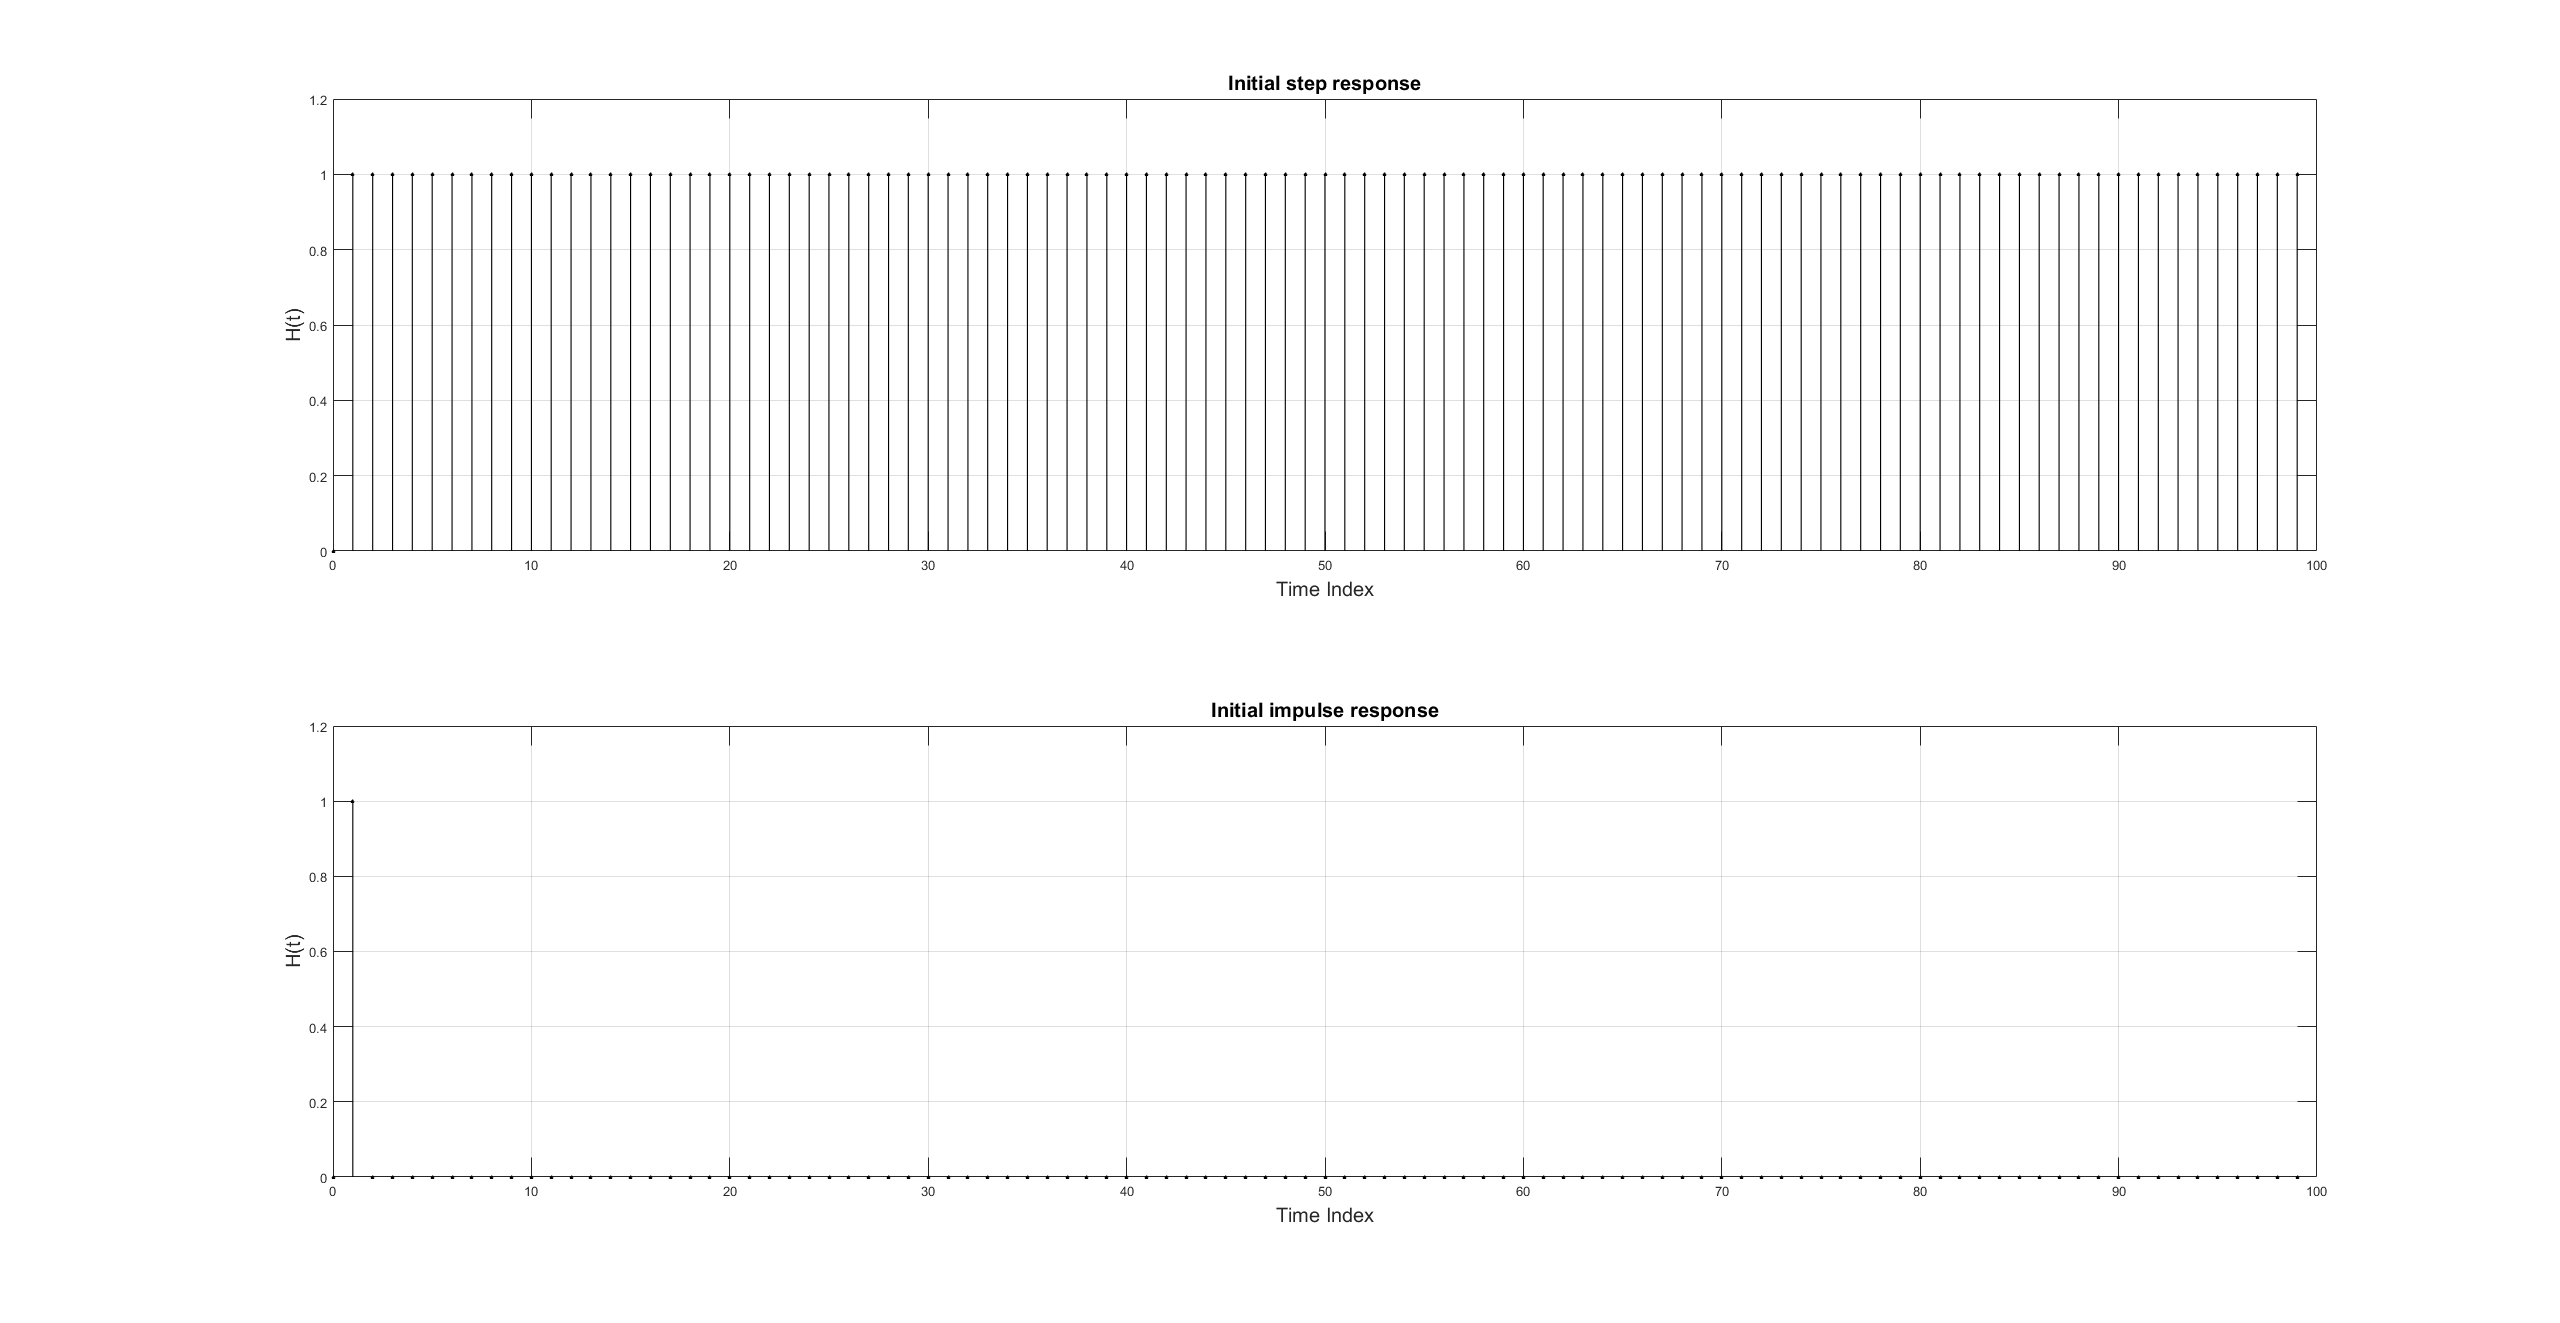
\includegraphics[width=\textwidth]{1.1.1.png}
		\caption{Input Impulse and Step Response}
		\label{figure:1_1_1}
	\end{figure}
	
	For the low pass signal response as seen in figure \ref{figure:1_1_2}, we see that the step response undergoes a time averaging affect as it takes a while for the filter to reach in the input signal, which is typical of a low pass filter. Similarly, the impulse response shows the effective settling time of the filter after an impulse, dependant on the filter coefficient.
	
	\begin{figure}[H] 
		\centering
		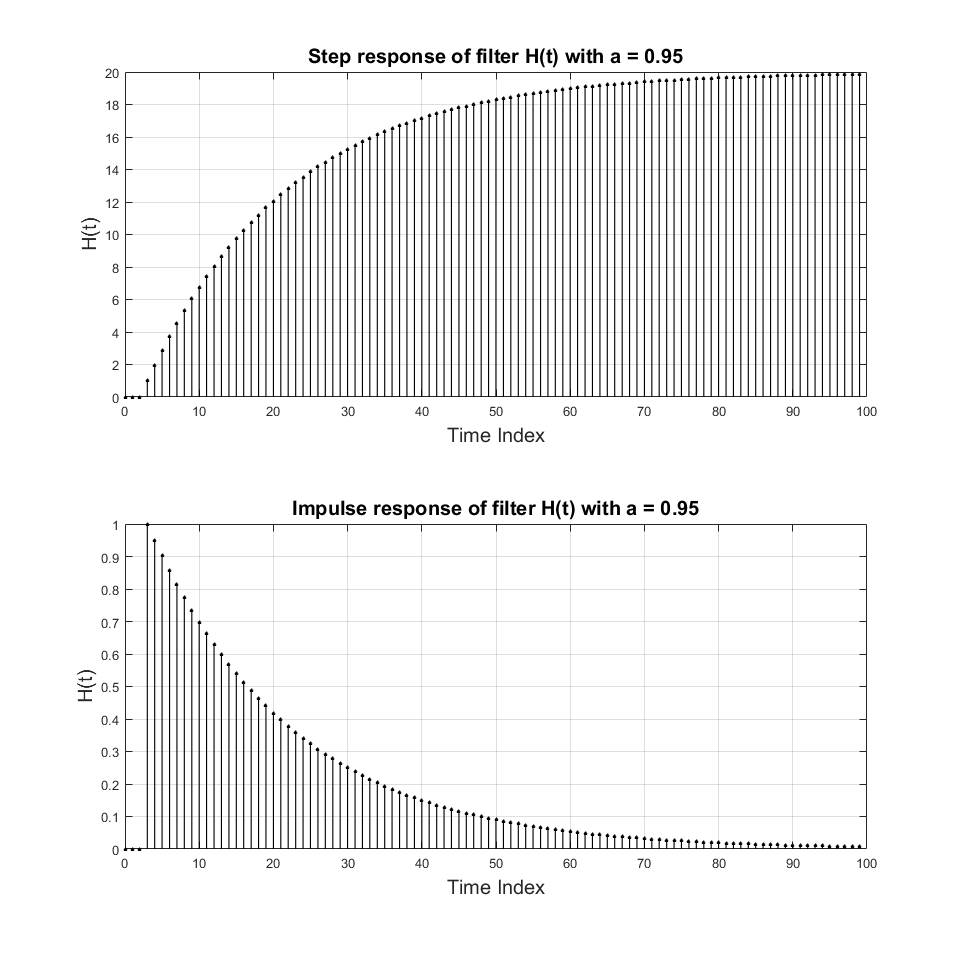
\includegraphics[width=\textwidth]{1.1.2.png}
		\caption{Low Pass Filter Response with a=0.95}
		\label{figure:1_1_2}
	\end{figure}

	For the high pass signal response as seen in figure \ref{figure:1_1_3}, we see that the difference in signal for the step response is magnified greatly, and that the initial rise time of the filter is instant. The impulse signal results shows an oscillatory behaviour, as the high frequency components of the impulse are greatly magnified, but not dampened.
	
	\begin{figure}[H] 
		\centering
		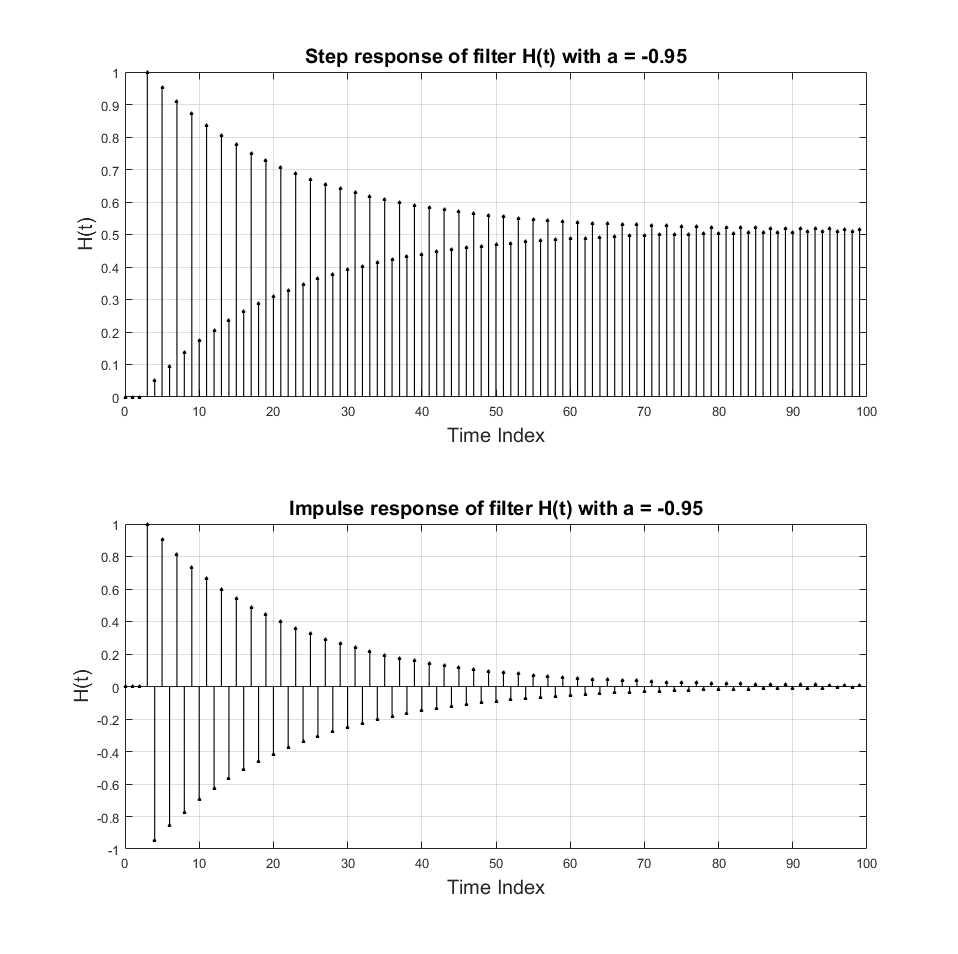
\includegraphics[width=\textwidth]{1.1.3.png}
		\caption{High Pass Filter Response with a=-0.95}
		\label{figure:1_1_3}
	\end{figure}